\chapter{Theoretical Framework}
\label{chapter:theoretical-framework}


This chapter describes the theoretical concepts needed to understand the work that will be developed during the research's execution.


\section{FER}

\section{Visual Transformer}

\section{Concept 1}

\label{section:Concept1}

First theoretical framework concept goes here.

\subsection{Subsection of Concept 1} 
\subsection{Subsection 2 of Concept 1}
Some text goes here \cite{examplereference}. An example of displaying and referencing an image is shown in \textbf{Figure \ref{fig:example}}


\begin{figure}
	\begin{center}
		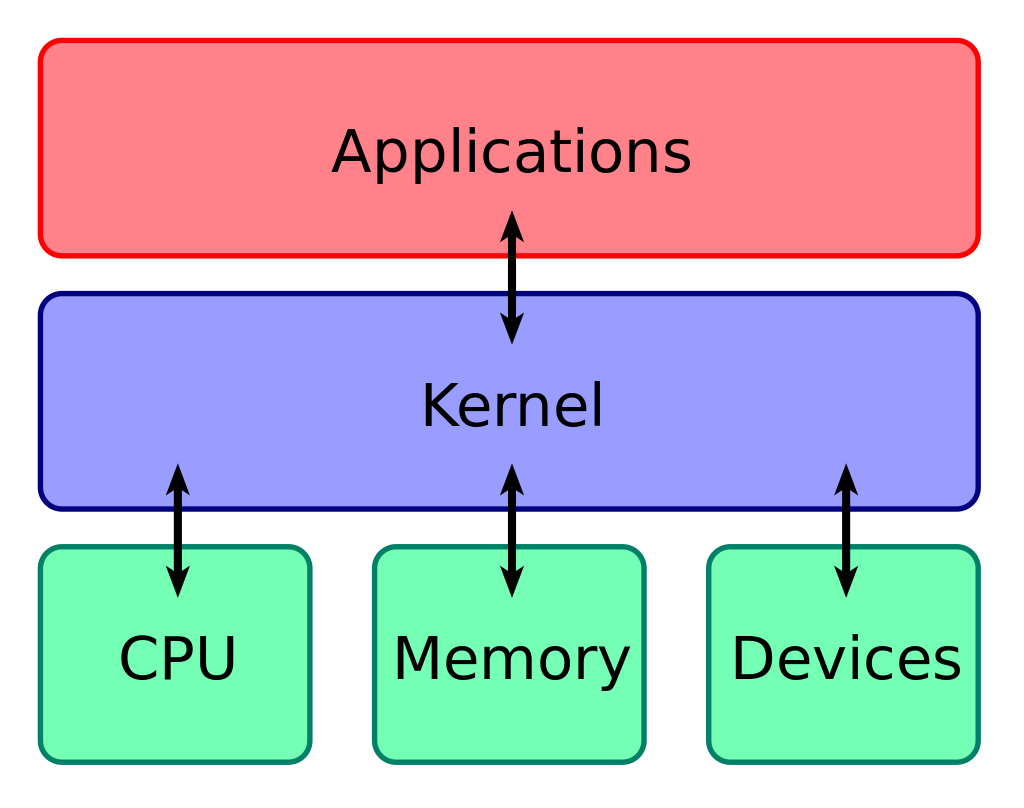
\includegraphics[width=1\columnwidth]{../img/image.png}
		\caption[]{Example image with reference \cite{examplereference}.}
		\label{fig:example}
	\end{center}
\end{figure}


\section{Concept 2}

\label{section:Concept2}

\subsection{Subsection Concept 2}

\subsubsection{Subsection 2 Concept 2}

\section{Concept 3}
An example of pseudo-code can be seen in \textbf{Algorithm \ref{examplepseudocode}}

\begin{pseudocode}{Pseudo\_Code}{Input} \label{examplepseudocode}
	\FOR y \GETS 1 \TO Input.MaxL \DO
	\BEGIN
	\FOR x \GETS 1 \TO Input.MaxH \DO
	\BEGIN
	a \GETS \CALL {FunctionCall}{x,y}\\
	b \GETS \CALL {AnotherFunction}{x, y}\\
	\CALL {ThirdFunction}{a,b}
	\END
	\END
\end{pseudocode}


\subsection{Example equation}
 Equation \ref{eq:1} shows an example equation.

\[
I=(L\cdot N) \tag{1} \label{eq:1}
\]
  
\section{Related Work}
The related work for the research is include in this section \cite{examplereference}.
